\documentclass[Visionprosjekt.tex]{subfiles} 
\NormalTopp
\begin{document} 

%%%%%%%%%%%%%%%%%%%%%%%%%%%%%%%%%%%%%%%%%%%%%%%%
\section{Feltbussystem}
\label{sec:feltbuss}
%%%%%%%%%%%%%%%%%%%%%%%%%%%%%%%%%%%%%%%%%%%%%%%%





En feltbuss er en metode for å kople sammen prosess- og automatiseringsutstyr i et «intelligent» nettverk med en felles kommunikasjonsprotokoll. Nettverket kan også tilføre feltutstyret drivspenning, f.eks. over Profibus PA.  Et feltbussystem gir en rekke fordeler, de viktigste er som følger \cite{FeltbussMortenPPT,veslemoy}.

\begin{itemize}
    \item Enklere og mindre kabling, noe som gir lavere kostnader.
    \item Standardisering; noder fra ulike produsenter kan benyttes om hverandre. Dette fører også til at det er god tilgang på feltbussutstyr.
    \item Mulighet for (selv-) diagnostisering.
    \item Smarte sensorer med f.eks. innebygd skalering og filtrering kan tilkobles og konfigureres via bussen.
    \item Bdere støyimmunitet enn ved vanlig analog overføring.
    \item Anlegget kan enkelt skaleres.
\end{itemize}




%•Protokoller : Communication Profiles ( DP, FMS, TCP/IP)


For kommunikasjon mellom PLS, I/O-modul og frekvensomformer, er  feltbussystemet Profibus DP benyttet, se \reff{fig:profiblokk}. Det neste underkapitlet vil beskrive Profibus DP nærmere.

\begin{figure}[ht]
	\centering
		%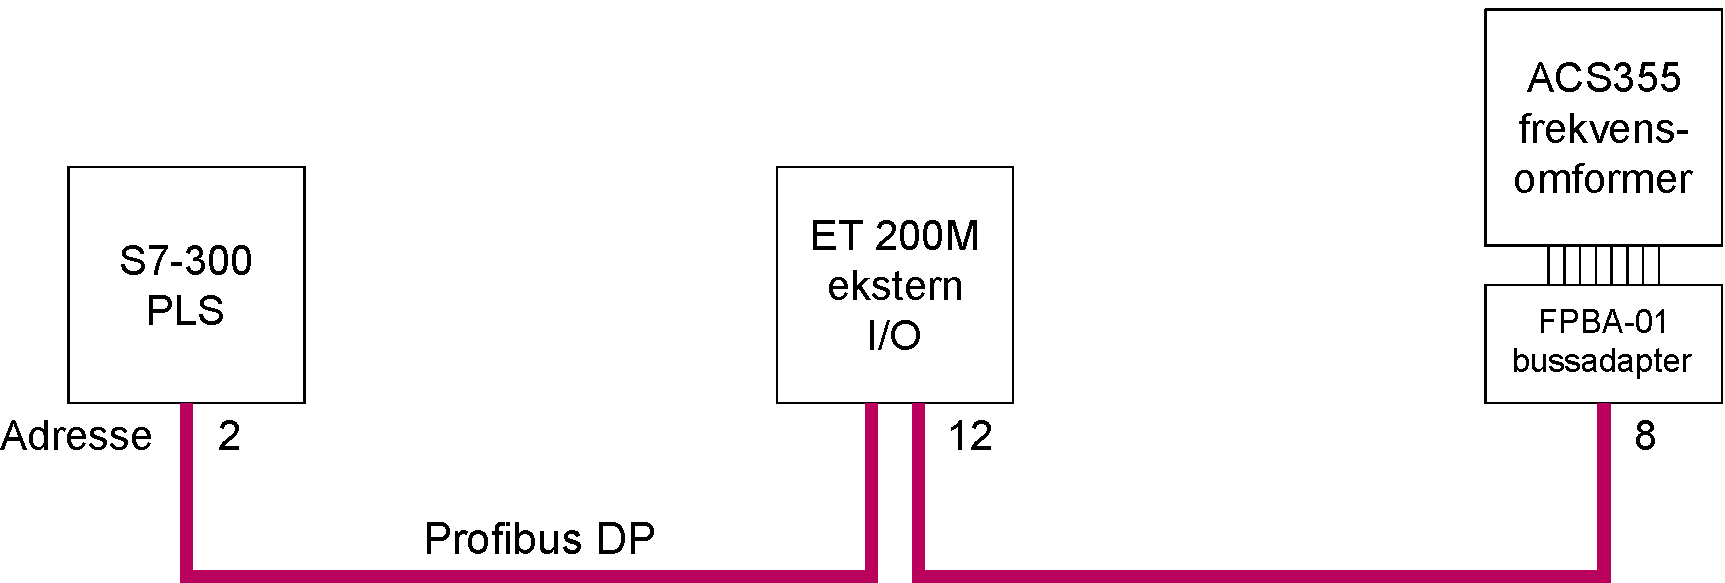
\includegraphics[width=0.8\textwidth,trim=0mm 0mm 0mm 90mm, clip=true]{bilder/profiblokk.pdf}
		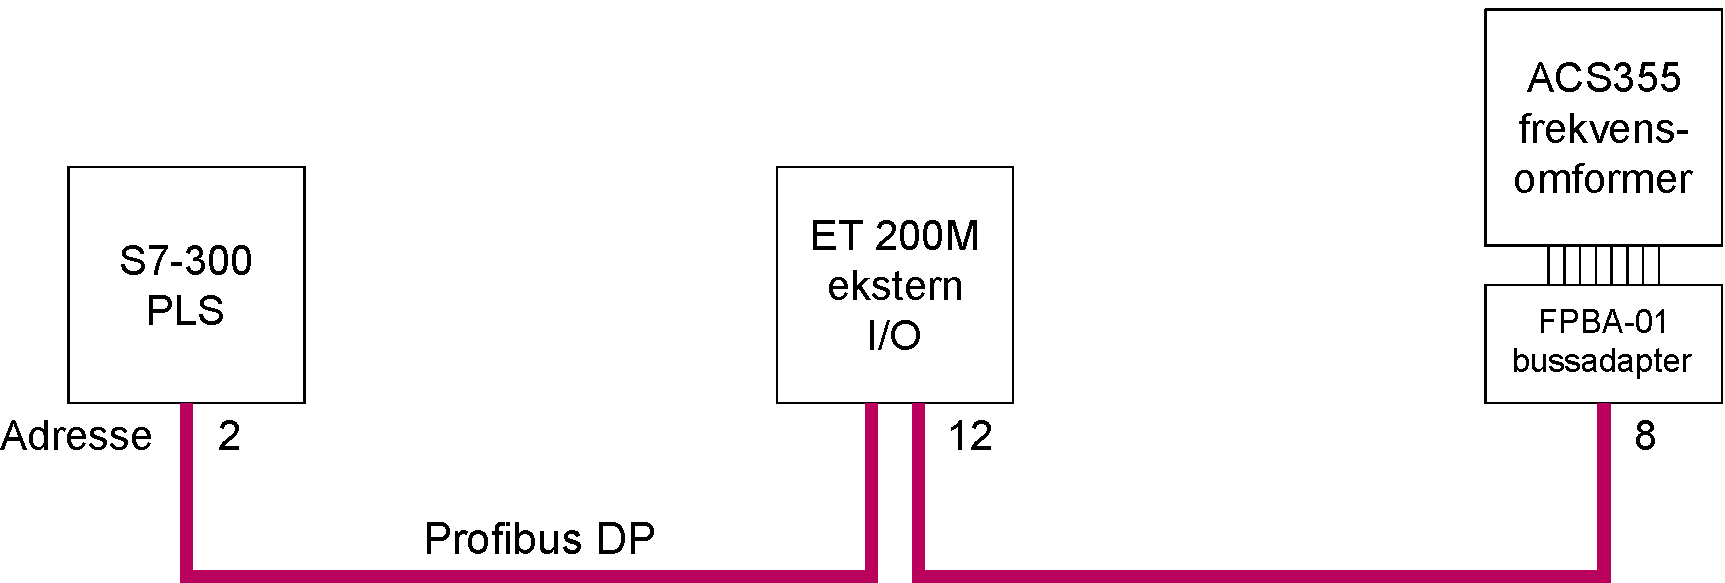
\includegraphics[width=0.8\textwidth]{bilder/profiblokk.pdf}
	\caption{Blokkdiagram for Profibus DP-systemet}
	\label{fig:profiblokk}
\end{figure}







%%%%%%%%%%%%%%%%%%%%%%%%%%%%%%%%%
\subsection{Profibus DP}
%%%%%%%%%%%%%%%%%%%%%%%%%%%%%%%%%

Feltbusstypen Profibus DP er en åpen standard definert i IEC 61158. I OSI-modellen finnes  Profibus på lag 1, 2 og 7. Hvert enkelt lag håndterer ulike deler av Profibus-standarden som følger \cite{ProfiStort,Skeienotat}.

\begin{itemize}
     \item Lag 1 (fysisk) definerer tre ulike media for overføring; kobberledning (RS485 eller MBP),  fiberoptisk kabel eller trådløs overføring. 
     \item Lag 2 (link/linje) definerer bussens aksessmetode; master/slave i kombinasjon med token. Her er også datasikkerhet implementert. 
     \item Lag 7 (applikasjon) definerer kommunikasjonsprotokollen Profibus DP. Denne finnes i tre ulike versjoner:
         \begin{itemize}
             \item DP-V0 for syklisk datautveksling og diagnostisering.
             \item DP-V1 for asyklisk og syklisk datautveksling og  alarmhåndtering.
             \item DP-V2 for datautveksling med faste tidsluker, såkalt «isochronous mode», og kommunikasjon mellom slaver. Her er det også mulighet for å kommunisere i «publisher/subscriber»-modus.
         \end{itemize}
\end{itemize}





%%%%%%%%%%%%%%%%%%%%%%%%%%%%%%%%%
\subsection{Konfigurasjon av Profibus DP-adapter}
%%%%%%%%%%%%%%%%%%%%%%%%%%%%%%%%%

For å få satt opp frekvensomformeren til å kommunisere over Profibus DP, må noen parametre forandres i frekvensomformerens og Profibus-adapterens innstillinger. Parameterne er spesifisert i \reft{tab:profibusparametre}. Noen parametre er ikke vist her, fordi de blir automatisk valgt. \cite{profibusadapter}


\begin{table}[ht]%
    \centering
    \caption{Parametre for feltbusskommunikasjon til frekvensomformer.}
    \label{tab:profibusparametre}
        \renewcommand\arraystretch{1.2}
    \begin{tabularx}{0.94\textwidth}{>{\ttfamily}l>{\ttfamily}l>{\raggedright\arraybackslash}X}
    \toprule
        \normalfont Parameter	& \normalfont Verdi	&	Beskrivelse\\
    \midrule
		1001 EXT1 COMMANDS		&	COMM		&	Gjør det mulig å starte og stoppe frekvens\-omformeren via feltbussen	\\
		1103 REF1 SELECT		&	COMM		&	Velger referansefrekvens \texttt{REF1}	\\
		1104 EXT REF1 MIN		&	0.0		&	Minimumsfrekvens som samsvarer med referanseord \\
		1105 EXT REF1 MAX		&	100.0	&	Maksimumsfrekvens som samsvarer med referanseord \\
		1601 RUN ENABLE		&	COMM		&	Velger feltbussen til å gi klarsignal til frekvens\-omformeren	\\
		1604 FAULT RESET SEL	&	COMM		&	Velger feltbussen til å kvittere feil		\\
          9802 COMM PROT SEL		&	EXT FBA	&	Aktiverer feltbusskommunikasjon				\\
          5102 FBA PAR 2			&	8		&	Adressen til frekvensomformeren på feltbuss-nettverket	\\
          5105 FBA PAR 5			&	1		&	Kommunikasjonsprofil						\\
          5127 FBA PAR REFRESH	&	REFRESH	&	Validerer feltbuss-parametre				\\
        \bottomrule
    \end{tabularx}
\end{table}

% 5102 NODE ADDRESS
% http://www.inverterdrive.com/file/ABB-FPBA-01-Profibus-Adapter-Manual/default.aspx







\end{document}